\chapter{Benutzerhandbuch}
Dieses Handbuch bezieht sich auf das UMVE Regioning-Plugin Version 1.0. Es enth\"alt detaillierte Anleitungen zum Ausf\"uhren bestimmter Funktionen mit diesem Plugin.

\section{\"Ubersicht}

\begin{figure}[h]
\centering
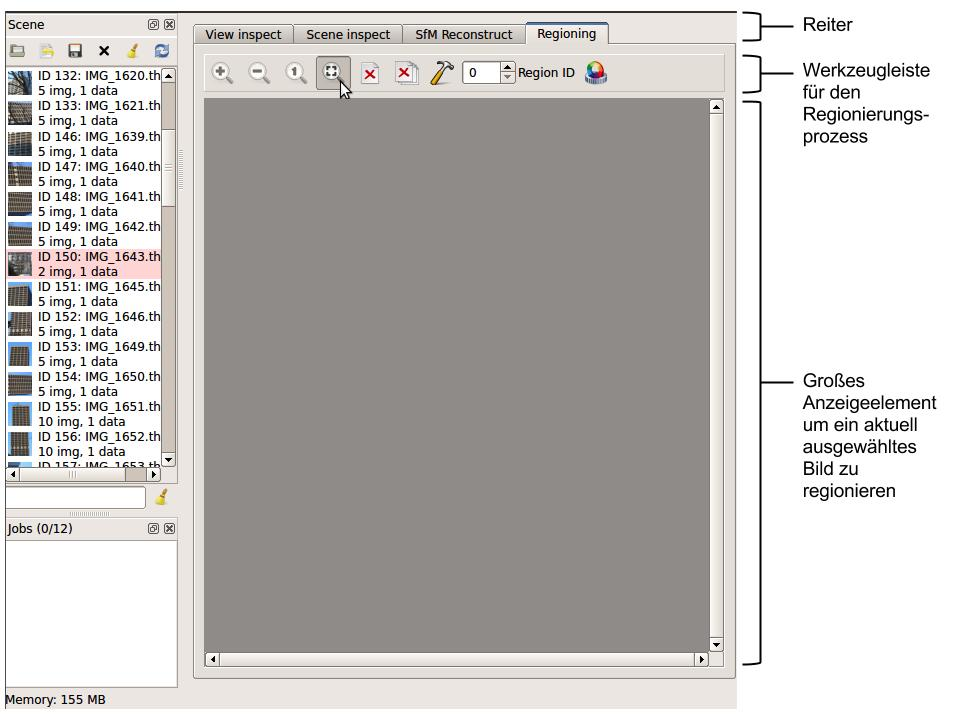
\includegraphics[width=0.9\textwidth]{gfx/Handbuch/RegioningPluginOverview.jpg}
\caption[\"Ubersicht \"uber das UI des Plugins]{\"Ubersicht \"uber das UI des Plugins}
\label{gr:uebersicht}
\end{figure}
\FloatBarrier

Das Plugin erscheint als zus\"atzlicher Reiter neben den bereits bestehenden (View inspect, Scene inspect, SfM Reconstruct) am oberen Rand des UMVE Fensters. Die Darstellung teilt sich hierbei einerseits in die Leiste mit den unterschiedlichen Werkzeugen und andererseits in die Anzeige der Bilddaten.

\section{Die Bildanzeige}
Das Plugin l\"asst sich \"uber die gewohnte Datenauswahl in der Scene am linken Rand steuern, sodass ein Klick auf das gew\"unschte Thumbnail gen\"ugt und das ausgew\"ahlte Bild erscheint in dem Anzeigeelement. Die Bildanzeige wird jeweils im Bearbeitungsmodus als auch im Regionierungsmodus verwendet und auch wie die Darstellung des aktuellen Bildes l\"asst sich dies \"uber die dar\"uber liegende Werkzeugleiste steuern (Hierzu mehr im folgenden Kapitel).

\newpage

\section{Werkzeuge und Arbeitsschritte}

\begin{figure}[h]
\centering

\includegraphics{gfx/Handbuch/toolbar.png}
\caption[Werkzeugleiste des Plugins]{Werkzeugleiste des Plugins}
\label{gr:toolbar}
\end{figure}
\FloatBarrier

Um die verschiedenen Werkzeuge zu verwenden, muss vorerst ein beliebiger Bilddatensatz ge\"offnet werden. Dabei werden unterschiedliche M\"oglichkeiten der Bilddarstellung und der Bearbeitung gezeigt.\\
Folgende Funktionalit\"aten stehen nun zur Verf\"ugung:\\
\begin{itemize}
\item \textbf{Vergr\"o\ss erungs- und Verkleinerungsfunktionen}

\begin{figure}[h]
\centering

\includegraphics{gfx/Handbuch/zoom.png}
\caption[Zoom-Funktionen des Plugins]{Zoom-Funktionen des Plugins}
\label{gr:zoom}
\end{figure}
\FloatBarrier

Mittels dieser Funktionen l\"asst sich, f\"ur eine genauere Regionsabgrenzung die Gr\"o\ss enansicht des Bildes regulieren. So sind die ersten beiden Symbole zur inkrementellen Vergr\"o\ss erung (einzoomen) als auch zur Verkleinerung (auszoomen). Eine verkleinerte Darstellung des Bildes ist n\"utzlich um einen \"Uberblick der bisherigen Regionierung zu sehen. Das dritte Lupensymbol, durch die \glqq 1\grqq \ gekennzeichnet, setzt den vorherigen Zoomfaktor wieder zur\"uck und zeigt das Bild in Originalgr\"o\ss e. Im Gegensatz dazu passt das vierte Symbol die Darstellung auf die Bildschirm- bzw. Fenstergr\"o\ss e an.
\newline
\item \textbf{Regionen entfernen}

\begin{figure}[h]
\centering
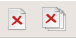
\includegraphics{gfx/Handbuch/delete.png}
\caption[L\"oschen-Funktionen des Plugins]{L\"oschen-Funktionen des Plugins}
\label{gr:loeschen}
\end{figure}
\FloatBarrier

Um bereits gezeichnete oder bearbeitete Regionen wieder zu l\"oschen gibt es diese beiden Funktionen. \"Uber die Region-ID Auswahl l\"asst sich eine zu l\"oschende ID ausw\"ahlen und durch das erste Symbol diese dann entfernen. Das zweite Symbol hingegen l\"oscht alle bestehenden Regionen aus dem aktuell ausgew\"ahlten Bild.
\newline
\newpage
\item \textbf{Regionierungs- und Bearbeitungsmodus}

\begin{figure}[h]
\centering
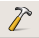
\includegraphics{gfx/Handbuch/edit.png}
\caption[Symbol zum \"Andern des Modus]{Symbol zum \"Andern des Modus}
\label{gr:modus}
\end{figure}
\FloatBarrier

Das Symbol ist zu Beginn nicht ausgew\"ahlt, was bedeutet, dass sich das Plugin im Regionierungsmodus befindet. \"Uber die linke Maustaste lassen sich nun beliebig viele Punkte setzen um eine Region abzugrenzen und mit der rechten Maustaste l\"asst sich schlie\ss lich das Polygon schlie\ss en. Vorrausetzung f\"ur diese Aktion ist, dass mindestens drei Punkte gesetzt wurden, die dann eine Fl\"ache aufspannen. Dazu wird der zuletzt gezeichnete Punkt mit dem ersten verbunden. Dabei spielt es keine Rolle, ob die Polygone konkav oder konvex gezeichnet sind. Wird eine zweite Region mit bereits existierender ID neu gezeichnet, so wird die erste entfernt und ersetzt. \\
Ist dieses Hammersymbol ausgew\"ahlt befindet sich das Plugin im Bearbeitungsmodus. \"Uber die Region-ID l\"asst sich hierf\"ur die zu bearbeitende Region ausw\"ahlen. Um die Form eines Polygons zu ver\"andern wird mit der linken Maustaste an die Stelle im Bild geklickt, zu der sich die bestehende Region ausdehnen bzw. verringern soll. Da kein expliziter Eckpunkt bestimmt wird, der seine Position ver\"andern soll, wird der Punkt gew\"ahlt, der der neu bestimmten Position am n\"achsten ist.
\newline
\item \textbf{Regions-ID Auswahl}

\begin{figure}[h]
\centering
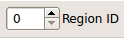
\includegraphics{gfx/Handbuch/regionID.png}
\caption[Regions-ID Auswahlfeld des Plugins]{Regions-ID Auswahlfeld des Plugins}
\label{gr:auswahl}
\end{figure}
\FloatBarrier

Diese Funktion wird nicht nur beim Zeichnen verwendet um der momentanen Region eine ID zuzuweisen, sondern auch bei den vorher beschriebenen Optionen. So muss die gew\"unschte ID gew\"ahlt werden, wenn eine bestimmte Region gel\"oscht oder bearbeitet werden soll. Wichtig ist, dass es maximal 8 verschiedene Regionen geben kann, wobei jede einzelne eine feste Farbzuweisung hat.
\newline
\item \textbf{Farbzuweisung der Regions-IDs}

\begin{figure}[h]
\centering

\includegraphics{gfx/Handbuch/chroma.png}
\caption[Farbzuweisungssymbol des Plugins]{Farbzuweisungssymbol des Plugins}
\label{gr:chroma}
\end{figure}
\FloatBarrier

Diese Funktion dient eigentlich nicht der Regionierung selbst, sondern \"offnet ein separates Fenster. Dieses zeigt eine Zuweisung der verwendeten Farben zu den zugeh\"origen IDs. Die Farbvergabe ist vorgegeben und beschr\"ankt die Anzahl verschiedener Regionen auf acht.

\begin{figure}[h]
\centering
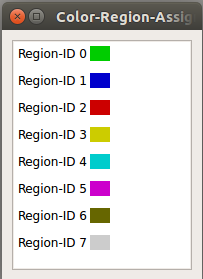
\includegraphics{gfx/cols.png}
\caption[Regions-ID-Farbzuweisung des Plugins]{Regions-ID-Farbzuweisung des Plugins}
\label{gr:zuweisung}
\end{figure}
\FloatBarrier

\end{itemize}

\section{Automatische Speicherfunktion}
F\"ur das anschlie\ss ende Matchingverfahren m\"ussen die Regionierungsparameter verf\"ugbar gemacht werden. Dazu m\"ussen gezeichnete Regionen in das vorgesehene Dateiformat geschrieben werden. Um Situationen zu vermeiden, in denen gezeichnete Regionen oder Ver\"anderungen vergessen werden zu speichern oder bei einem Bildwechsel verloren gehen, existiert eine automatische Speicherfunktion. Das automatische Speichern betrifft hierbei folgende Aktionen:\\
\begin{itemize}
\item Das Einzeichnen und Abschlie\ss en einzelner Regionen
\item Das Bearbeiten einzelner Regionen
\item Das L\"oschen einzelner oder aller Regionen
\end{itemize}
Jede einzelne Modifikation der Regionierungsparameter wird festgehalten, sodass eine manuelle Speicherung entf\"allt und man bedenkenlos nach Fertigstellung der Regionierung das n\"achste Bild \"offnen kann.